\documentclass[12pt,letterpaper]{article}
\usepackage[utf8]{inputenx} %Codificacion del texto (ISO Latin1 encoding)

\usepackage{fancyhdr} %Permite acomodar a tu gusto la parte de arriba y
% abajo del documento
\usepackage[spanish]{babel} %Permite definir el idioma del dcumento
\usepackage{graphicx} %Permite exportar imagenes en formato eps
\usepackage{url} %Tipo de fuente para correos y paginas
\usepackage{pgf}
\usepackage{fleqn}
\usepackage{amssymb}
\usepackage{amsmath}
\usepackage{bigints}
\usepackage{fancyvrb}
\usepackage{makeidx}
\usepackage{colortbl} %Permite colocar colores a las tablas
\usepackage{multirow}
\usepackage{booktabs}
\usepackage{moreverb}
\usepackage{rotating}
\usepackage{lastpage}
\usepackage[final]{pdfpages}
%%%%%%%%%%
%Margenes%
%%%%%%%%%%
\usepackage[top=3cm,bottom=3cm,left=3cm,right=3cm,footskip=1.5cm,headheight=1.5cm,headsep=.5cm,textheight=3cm]{geometry}
%%%%%%%%%%%%%%%%%%%%%%
%Estilo del documento%
%%%%%%%%%%%%%%%%%%%%%%
\pagestyle{fancyplain}

%%%%%%%%%%%%%%%%%%%%%%%%%%%%%%%%%%%%%%%%%%%
%Fancyheadings. Top y Bottom del documento%
%%%%%%%%%%%%%%%%%%%%%%%%%%%%%%%%%%%%%%%%%%%
% Recuerde que en este documento la portada del documento no posee
% numeracion, pero de igual manera llamaremos a esa primera pagina la numero
% 1, y la que viene la dos. Esto es para tener una idea de las que
% llamaremos pares e impares
\lhead{Laboratorio mat024} %Parte superior izquierda
\rhead{\bf \it Preinforme 2} %Parte superior derecha
\lfoot{\it Victor Gonzalez} %Parte inferior izquierda. \thepage indica
% el numero de pagina
\cfoot{\bf \thepage} %Parte inferior central
\rfoot{página \thepage\ de \pageref{LastPage}} %Parte inferior derecha
\renewcommand{\footrulewidth}{0.4pt} %Linea de separacion inferior

\begin{document}
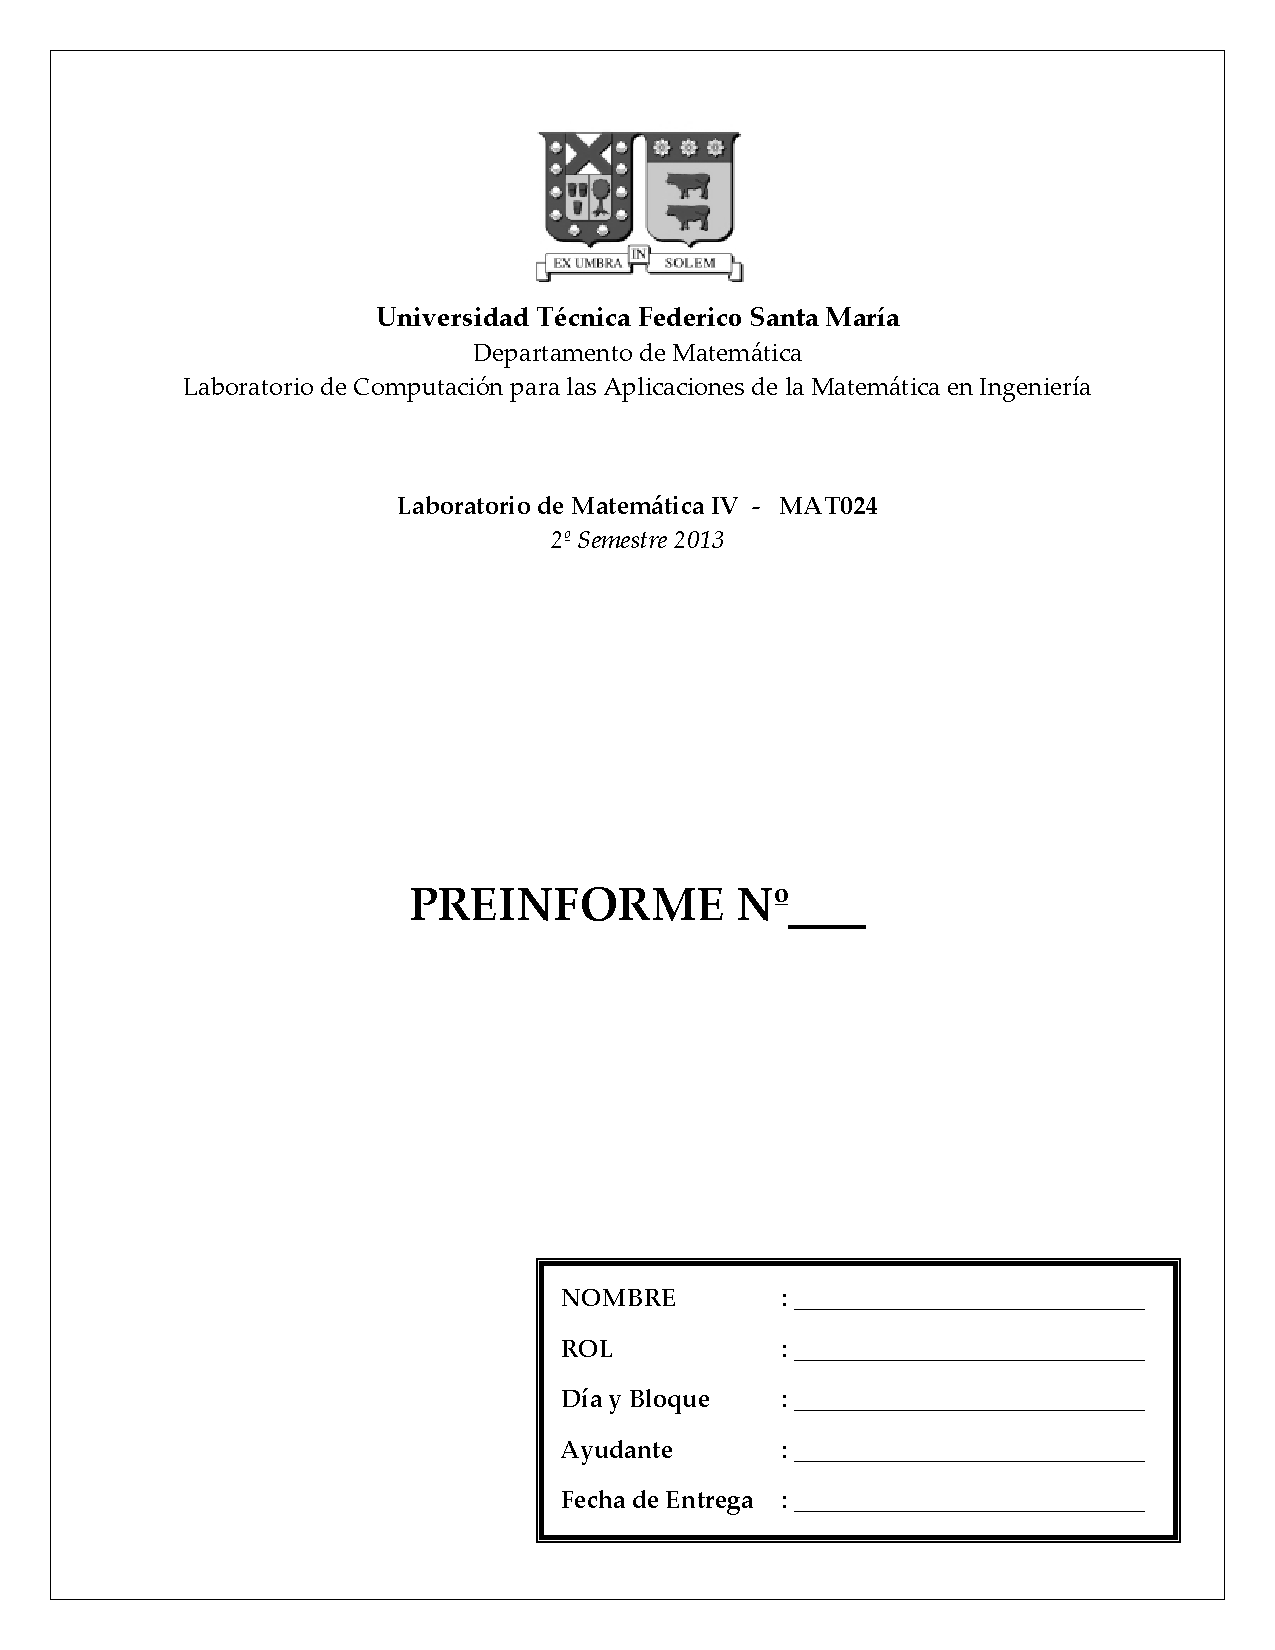
\includepdf[pages={1}]{portada.pdf}

\section{Desarrollo Analítico y Planteamiento}
Para el resto del documento considerar $\alpha=4$ y $\beta=9$.
\subsection{Pregunta 1}
\subsubsection{Parte a}
La curva $C$, es la intersección entre la superficie $S_1: z-2=x+\beta$ y la superficie $S_2: 4z=x^2+ (y- \alpha)^2$.

Luego, la intersección de ambas se puede hacer despejando $z$ desde $S_1$, para luego reemplazarlo en $S_2$, lo cual entrega la figura en el plano x-y:

\begin{center}$C: \dfrac{(x-2)^2}{\sqrt{48}^2} + \dfrac{(y-4)^2}{\sqrt{48}^2}=1$\end{center}

Lo cual corresponde a una elipse centrada en $\{2,4\}$. En el anexo, se puede observar en la \textit{figura 2}, la intersección de los 2 planos, y efectivamente la elipse generada al intersectarse estos 2 planos.

Luego, procedemos a parametrizar esta elipse, haciendo el siguiente cambio de variables: $x=2+\sqrt{48}Cos(t)$, $y=4+\sqrt{48}Sin(t)$, donde $0\leq t \leq 2\pi$.

Por lo tanto, la función parametrizada es:

\begin{center}$r(t)=\{2+\sqrt{48}Cos(t),4+\sqrt{48}Sin(t),2+2+\sqrt{48}Cos(t)+\beta \}$\end{center}

Se puede observar en la \textit{figura 1} del anexo, la gráfica de la parametrización, la cual es la misma que la de la presentada previamente.

Finalmente, para calcular la longitud de esta curva, se aplica la integral:

\begin{center}$\bigints_0^{2\pi} \! \sqrt{(\frac{dx}{dt})^2+(\frac{dy}{dt})^2+(\frac{dz}{dt})^2} dt$\end{center}

La cual da por resultado $52.9342$.

\subsubsection{Parte b}
Para calcular la masa, basta usar la integral de longitud e introducir la densidad dentro del integrando, dejando la integral de masa de la siguiente forma:

\begin{center}$\bigints_0^{2\pi} \! (x^2+y^2+z^2)\sqrt{(\frac{dx}{dt})^2+(\frac{dy}{dt})^2+(\frac{dz}{dt})^2} dt$\end{center}

Lo cual, luego de aplicar los cambios de variables del ejercicio anterior, entrega por resultado $13708$.

\subsection{Pregunta 2}
\subsubsection{Parte a}
Se nos pide verificar que $\nabla f= \vec{F}$, donde:

\begin{center}$f(x,y)=\frac{1}{2}\bigintsss_a^{x^2+y^2} \!\!\!\! g(t)dt$\end{center}
\begin{center}$\vec{F}(x,y)=(xg(x^2+y^2),yg(x^2+y^2))$\end{center}

Luego, el gradiente de $f$, viene dado por $\nabla f = \left\{\dfrac{df}{dx},\dfrac{df}{dx}\right\}$, el cual es\\ $\nabla f = \left\{xg(x^2+y^2),yg(x^2+y^2)\right\}$.\\

Por lo tanto, es correcto afirmar que $\nabla f= \vec{F}$. Esto es verificado en \textit{Mathematica}, y puede ser obvservado en la sección de la pregunta 2, parte a.

\subsubsection{Parte b}
Se nos pide calcular la integral: $\bigoints_C \dfrac{xdx}{(x^2+y^2)^{\alpha+3}} + \dfrac{ydy}{(x^2+y^2)^{\alpha+3}}$, sobre la curva \\ $C: \{Cos^4(t),4Sin^3(t)\}$.\\

Sea $\vec{F}=\left(P\rightarrow\dfrac{x}{(x^2+y^2)^{\alpha+3}},Q\rightarrow\dfrac{y}{(x^2+y^2)^{\alpha+3}}\right)$. Notamos que $\vec{F}$ no es $C^1$ en $\mathbb{R}^2$ pero si lo es cuando tenemos $\mathbb{R}^2 / {(0,0)}$. Por lo tanto, podemos utilizar el teorema de Green para encerrar ese pequeño agujero en el dominio, para asi recorrer dominios multiplemente conexos.

Al verificar el valor del rotacional $\dfrac{dQ}{dx}-\dfrac{dP}{dy}$, obtenemos un cero, por lo que basta obtener la integral sobre el círculo de radio $\epsilon$ ($\gamma_\epsilon$), que cubre la indeterminación en $(0,0)$:

\begin{center}$\bigoints_C \dfrac{xdx}{(x^2+y^2)^{\alpha+3}} + \dfrac{ydy}{(x^2+y^2)^{\alpha+3}} = \dfrac{1}{\epsilon^{14}}\bigoints_{\gamma_\epsilon} xdx+ydy$\end{center}

Luego, al aplicar la parametrización del círculo de radio $\epsilon$ obtenemos finalmente, que el resultado es 0.

\subsection{Pregunta 3}
Se nos pide calcular la integral $\bigintss_{C_1} (xe^{x^2}-3y)dx + (\beta+2x+yCos(y^2))dy$, donde $C_1$ es el triángulo equilatero con solo 2 lados.

Sea $\vec{F}(x,y)=(P\rightarrow xe^{x^2}-3y,Q\rightarrow\beta+2x+yCos(y^2))$. El rotacional $\dfrac{dQ}{dx}-\dfrac{dP}{dy}$ es $5$, por lo tanto nuestra integral queda como la suma de otras 2 integrales:

\begin{center}$\bigints_0^{\sqrt{12}}\bigints_{\frac{2x}{\sqrt{12}}}^{\frac{-2x}{\sqrt{12}}+\alpha} 5dydx + \bigints_0^{\alpha}(\beta+2x+yCos(x^2))dx$\end{center}

Luego, esta suma de integrales, deja por concluir que

 $\bigintss_{C_1} (xe^{x^2}-3y)dx + (\beta+2x+yCos(y^2))dy = 70.4971$.
\section{Conclusiones}

Las integrales de linea, resultan ser unas de las aplicaciones mas prácticas de las matemáticas avanzadas, dada su estrecha relación con la física. Donde podemos calcular mediante modelos matemáticos, las longitudes o masas de complejas figuras geométricas.

Por otro lado, el Teorema de Green resulta ser una gran ayuda cuando tenemos problemas con el dominio donde queremos integrar, ya que mediante ciertos pasos, logramos sortear problemas complejos de resolver, entregando una herramienta util al momento de cubrir dominios.

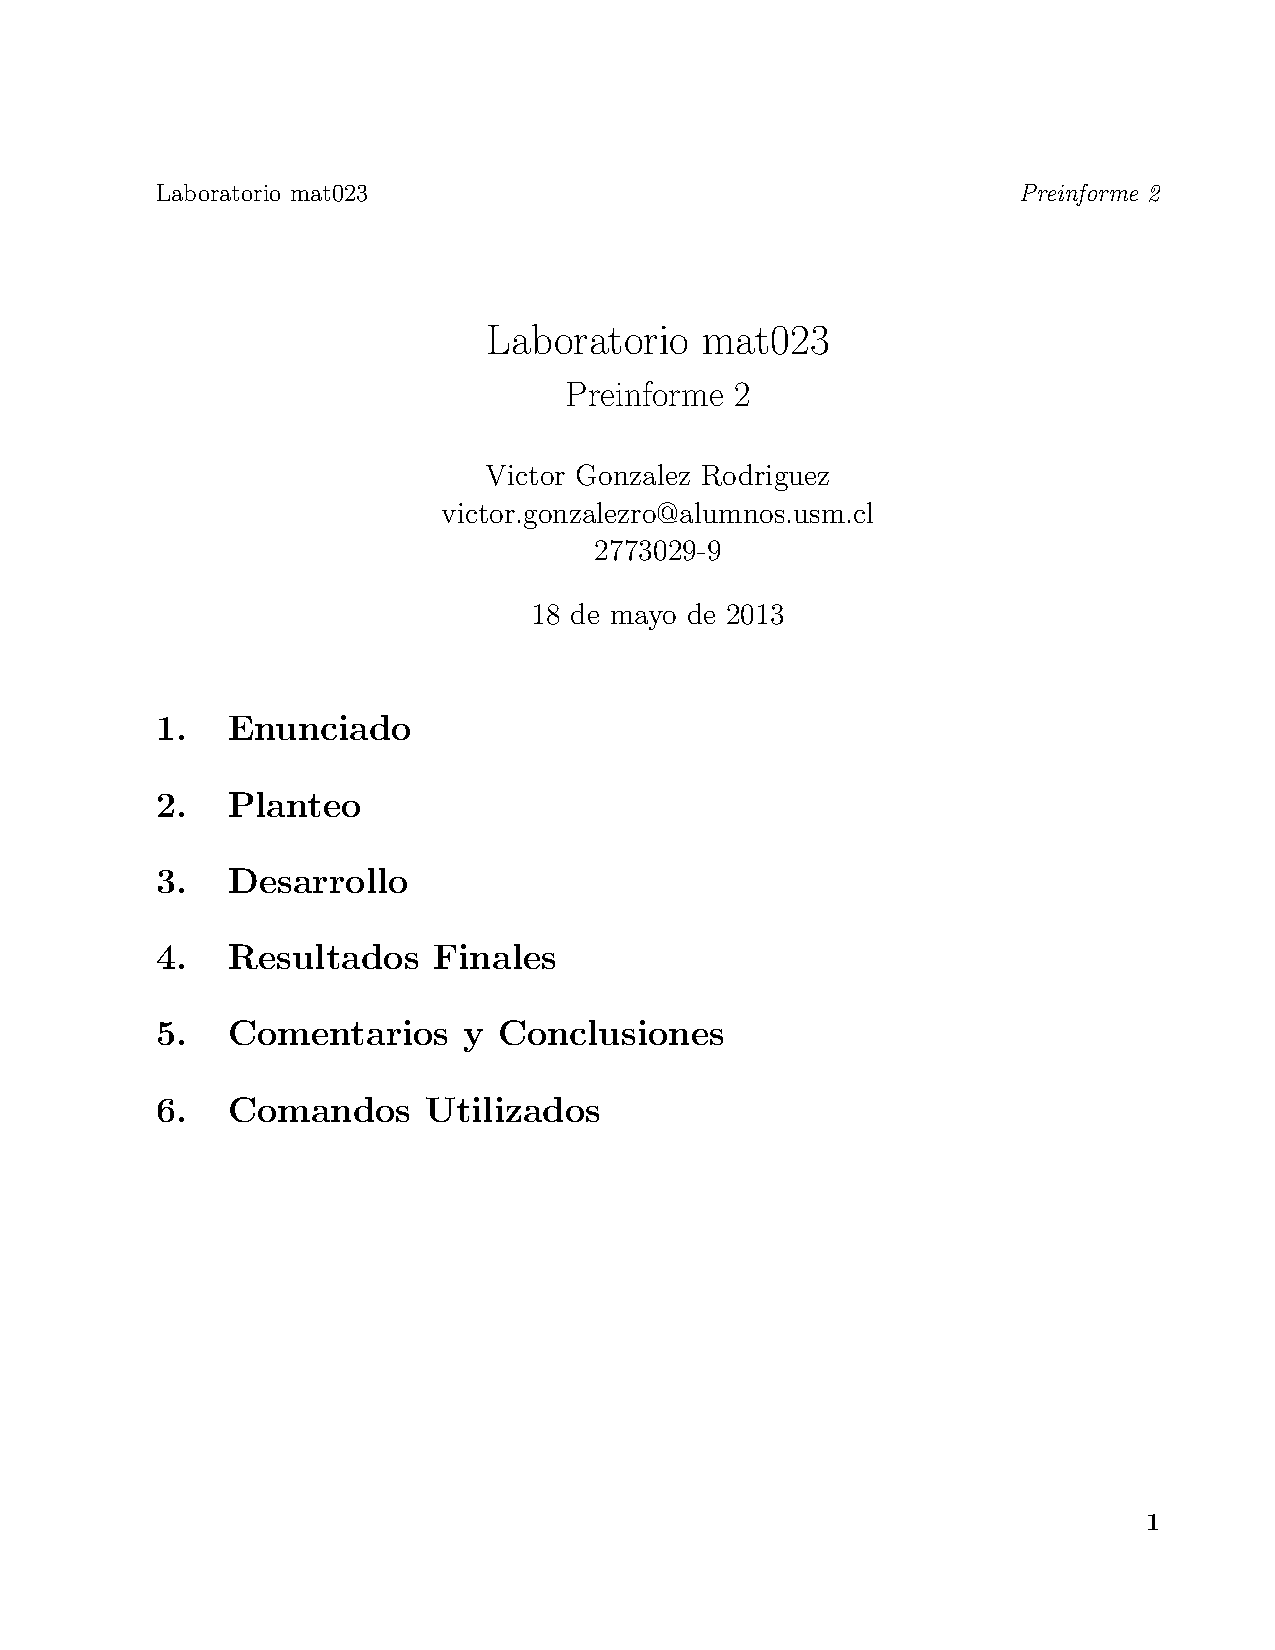
\includepdf[pages={1,2,3,4,5}]{lab2.pdf}

\end{document}